\documentclass{report}
\usepackage{graphicx}
\usepackage[hidelinks]{hyperref}
\usepackage{cite}
\begin{document}
\begin{titlepage}
    \begin{center}
        \vspace{1.0cm}
        
\includegraphics[scale=0.5]{Warwick}
        \vspace*{1cm}
  
        % Title
        \textbf{Using Ad Hoc Networking in Emergency Situations}
  
        \vspace{0.5cm}
        % Subtitle
        Spreading information in an emergency situation to help both people in danger and the emergency services
  
        \vspace{1.5cm}

        % What the project is about
        \textbf{Project Specification}
  
        \vspace{1.6cm}

        % Author name
        \textbf{Freddie Brown}\\
        \textbf{u1716717}


  
        \vspace{1.6cm}
        % Information about the institution
        Supervisor: Dr. Matthew Leeke\\
        Department of Computer Science\\
        University of Warwick\\
        2019-20
  
    \end{center}
\end{titlepage}


\chapter*{Abstract}
% \pagenumbering{roman}
\addcontentsline{toc}{chapter}{Abstract}

When an emergency situation occurs, people want to tell others where they are and get help. 
This can often be difficult to do because key infrastructure that is heavily relied on could be damaged.
Situations around the world show there is a significant need for systems to help peope connect with no, or very little, working cellular infrastructure. 
By using commodity hardware in our devices, survivors can oppurtunistically send information to nearby devices. 
This could then be sent to an internet connected device for transmission, other nearby devices or, the emergency services. 
Moving information in emergency situations could get alert those who save lives and could aid rescue efforts.
\\
\\
\textit{Keywords: Bluetooth, Ad Hoc, MANET, Emergency, Disaster}


% \chapter*{Acknowledgements}
% \addcontentsline{toc}{chapter}{Acknowledgements}
% Acknowledgements

\chapter*{Abbreviations}
\addcontentsline{toc}{chapter}{Abbreviations}

\textbf{MANET} - Mobile Ad Hoc Network\\
\textbf{VM} - Virtual Machine\\
\textbf{BCS} - British Computing Society\\
\textbf{WSN} - Wireless Sensor Network\\



% \tableofcontents{}

\chapter*{Introduction}
% \pagenumbering{arabic}

The main part of this project is investigating the application of MANETs for emergency situations, an interesting technology which could be used
effectively for emergency situations. They are low infrastructure networks which use homogenous and heterogenous devices to form a 
network dynamically. This is incredibly interesting in situations which are quite fluid, with nodes coming in and out of a network\cite{sun2001mobile}. 
There are some other areas which this project will also explore, such as keeping devices alive for a long time, biological 
inspired routing and security issues related to passing packets of potentially sensitive data to unverified devices to distribute. These areas complement 
the main project problem as they help to solve some questions associated with MANETs in this context.


\section*{Motivations}
In todays world, most people in the world rely on telecommunications to connect with family members, friends, 
work collegues and, very importantly, the emergency services. When we get a disaster, or group of them, as was 
seen in Puerto Rico in 2017, it can impact lives and even end them prematurely. A study estimates the increase in 
mortality of 62\%\cite{kishore2018mortality}, and this is thought to be an underestimate. Remote areas were hit hardest and were without services 
such as cellular data access for up to 41 days. This can make it very difficult for rescuers to know the situation in 
these places and creates a mismatch in information. This is a common cause of high cost and disrupsion in many different disasters. 
Another example of this was in Hurricane Katrina\cite{banipal2006strategic} where high winds saw antennas, belonging to celluar 
providers, highly damaged or destroyed. 
\bigskip\\
Incidents such as these illustrate the tragic consequences that can happen without vital services which are required in the 
world today. In 2016, the United Nations voted that access to the internet is a human right that should be protected\cite{UNResolutionJune2016}. 
This type of action brings into focus the need to have systems in place to help people maintain connectivity, even when traditional infrastructure 
fails. 

\section*{Project Aims}

The aim of the project is to produce a prototype of a system which could be implemented by governments and technology 
companies which could help people. Companies like Google and Apple produce the Operating Systems for most phones but 
they don't have any sort of inbuilt emergency system like the one I hope to accomplish. 
\bigskip\\
I want to explore the different ways this could be implemented, what holds them back and how well they actually perform 
in action. Also, I want looking at why there is no widely implemented system such as this in consumer phones already. 

\section*{Stakeholders}

The stakeholders for this project would be those who can benefit from it. Those people are those who live in areas 
which are frequently affected by natural disaster and have weak infrastructure. These are the people that would benefit 
most from having a system which could help them maintain contact with the world if they couldn't through traditional 
methods.

\chapter*{Research}

\section*{Different Implementations}

Although this is still an open problem, there have been a few different implementations and ideas about similar systems. One such example is 
HIRO-NET\cite{ferranti2019hiro}. In this example, the approach looks at 2 tiers. One tier is looking at local meshing, similar to this project, 
and the other tier is looking at connecting these mesh networks over a larger area. The local meshing uses Bluetooth Low Energy to connect 
devices together and sticks to a Client-Server model. Each server will start off as a client. If it cannot find any nearby server, it will then 
become a server and start advertising as such. If another server then appears, they will join together their piconets to form a scatternet 
to increase the number of connected devices. Also, server declare if their piconet is connected to the internet so that other servers can route 
pakcets to it to send out beyond the local mesh. The main aim of this is to allow devices to maintain a regular internet connection to allow them 
access to normal internet services such as social media. 
\bigskip\\
Another approach focuses on getting emergency information out to the emergency services\cite{wu2011emergency}. This approach is a lot more simple than 
HIRO-NET as its sole focus is taking an emergency message, such as geographical information, and transporting it to an operational base to allow rescuers 
to find people who are in trouble. This proposed system investigates the use of both WiFi and Bluetooth in an emergency communications system and how they 
can both play an important role together. The conclusion in this research is that, because WiFi has a longer range and is a more widely available technology, 
it plays a more important role than Bluetooth is spreading emergency information. 
\bigskip\\
WiFi is a very important and very useful technology becuase of its long-range, for example, 802.11p can reach up to 1,000m \cite{abdelgader2014physical} whereas Bluetooth
is typically used for shorter ranges. This is discussed in \cite{bhagwat2001bluetooth}. Despite this, when there is a scenario 
where devices are going to be without a large power source for a long time, it could be more power efficient to use Bluetooth\cite{putra2017comparison}, although some 
dispute this \cite{friedman2012power} so it is good to consider both technologies. For this reason, looking at Bluetooth WSN systems could provide good inspiration for 
how to build the system. A system presented by Chu et al \cite{chu2010design} shows a high performance sensor network system. Although it uses highly optimised hardware 
to accomplish the task (which is different to the system this project is investigating), it presents ways for nodes to work more efficiently, such as only having 1 
route to send outgoing traffic. It also presents how the WSN is formed and the role of each node. 

\section*{Data Privacy}

Data privacy is a necessary, important, and highly sensitive topic which has legal ramifications if ignored. It is especially important in this project because it will 
deal with information which, if in the wrong hands, could harm someones wellbeing. For this to be effective, any solution needs to ensure confidentiality and integrity of the data.
\bigskip\\
One way to do this might be to use Diffie–Hellman key exchange\cite{li2010research} \cite{diffie1976new} alongisde another symmetric key algorithm, which provides confidentiality. This DH is a well known way to do public key exchange over 
a public, interceptable channel like bluetooth. There are some drawbacks to this, such as user authentication, as presented by Li. This could be solved by using a digital 
certificate. This is prested by Diffie and Hellman in \cite{diffie1976new}. This provides integrity to the transmission. Another positive to this is that there doesn't need to be any keys stored over a long period of time. This reduces vulnerability to attack and makes solving 
each key by brute force a less attractive prospect. On the other hand, calculating it each time can be a computationally intensive process. This could waste valuable 
computational power, especially when there is a definite need to conserve power and use resources as effectively as possible. 
\bigskip\\
Another option could be to use public key encryption, such as RSA \cite{aufa2018security}. This is a highly secure method and is widely used. In a MANET, each node could 
broadcast its public key when it connects to the network, as an update. Each node could store this public key. Everytime a node wants to communicate with another node, it can 
encrypt the message with the receiving nodes key. This way the privacy of the message is maintained. To maintain integrity of the message, a digital signature could be 
used. 

\section*{Routing}

Due to the Client-Server model employed by Bluetooth systems, routing tends to be device to device. For this project, it will investigate connecting multiple piconets together 
and routing packets between devices wihtin the wider scatternet effectively. A good way to do this could be by using one of the many routing algorithms out there. Each one deals 
with different challenges and is applicable to different scenarios. 

\chapter*{Ethical, Social, Legal and Professional Issues}

\section*{Ethical Issues}

Ethical issues arise when there are competing goods and competing evils. An example of this 
is using data collected through using a product to target certain groups without their consent. 
A firm may make more money by doing this, but whether it is right to do so is something that 
should be considered. Fundamentally, stakeholders in the project should be protected and their 
data shouldn't be used against them. Data should be kept anonymous and protected somehow, through 
traditional encryption or other means. 

\section*{Social Issues}

Social issues are those that may have an affect on the lives of many people. It could be problems which 
affect how they interact with other people or those relating to access to goods and services that others can 
but they can't. Currently, it is hard to see any issues of this nature relating to the project but this should 
be continually considered as the project moves forward.

\section*{Legal Issues}

This project will deal with sending data about an individual to others and allowing them to hold and send this 
data to whomever they wish to send it to. There are legal issues as, without proper protections, this kind of 
data could be used against individuals that are in trouble, such as in a terror incident. 
\bigskip
\\
In this project, sensitive data will be dealt with appropriately, such as location data, so no one is privy to this 
information at any time if they shouldn't have access to it. As discussed above in Ethical Issues, this should be 
done by maintaining data privacy through encryption or other means.

\section*{Professional Issues}

This project will adhere to the BCS Code of Conduct\cite{BCSCoP}. The aim is to produce a 
research project which can be trusted and respected and so adherence to all rules that are required 
is important. This means I will also follow the Research Code of Practice at the University of Warwick\cite{UniWarwickCOP}. 
This means all work I use to support my research will be referenced. 

\chapter*{Project Requirements}

\section*{Functional}

\textbf{FR1} - The system must use a widely used MAC layer protocol such as Bluetooth or WiFi.\\
\textbf{FR2} - The system must have the capability to have nodes connected to the internet (sinks) as well as those which aren't (sources/routers).\\
\textbf{FR2.1} - Within the nodes not connected to the internet, there should be 2 types of node: Nodes of regular citizens(sources) and those belonging to the emergency services 
which can accept and deal with data like internet nodes (sinks).\\
\textbf{FR3} - The system must use a mechanism to enable data privacy within packets, such as encryption.\\
\textbf{FR4} - The system should consider the battery life and make choices to extend this as much as possible\\
\textbf{FR5} - The system must provide an API which can be implemented by other services.\\
\textbf{FR5.1} - This API must be simple to use so services can route traffic in disaster scenarios.\\

\section*{Non-Functional}

\textbf{NFR1} - The system must be fully documented and maintainable.\\
\textbf{NFR2} - The system must be easy for a user to connect to and use.\\
\textbf{NFR3} - The system must be created so it can be applied to a large population of devices.\\
\textbf{NFR4} - The system must be able to be used by different types of devices such as IoT as well as Phones, Tablets and PCs\\
\textbf{NFR5} - The system could provide a way for other services to use the network to send out internet traffic.\\

\section*{Constraints}

This project will be constrained by the number of devices which it can be tested on and the type of devices which can be used. Having access 
to lots of devices can be very expensive. This project will use Raspberry Pi's to demonstrate the application of the research but these cost 
money and it won't be able to replicate the scale at which an emergency situation may be.
\bigskip\\
A further constraint will be the types of devices. The research will focus on applications in a heterogenous network of devices but it is 
likely this will only be demonstrated on a homogenous network as more popular devices (e.g iOS and Android\cite{mobileOS}), which this type of system would be employed on in the 
real world, don't allow root access and are restrictive about what can be run on devices. This makes them difficult to develop for on this project, but are platforms which 
this would need be implemented on in the real world.

\chapter*{Project Management}

\section*{Project Timeline}

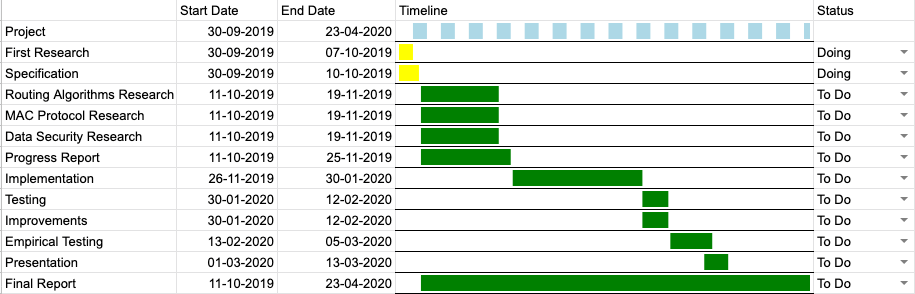
\includegraphics[scale=0.35]{ProjectTimeline}

\bigskip

The above figure shows the predicted project timeline in a Gantt chart as well as displaying the dates between 
which each task will take place. Looking at the timeline, ample time has been left for research for the different aspects of the 
project (about a month). During this time, the second project deliverable can also be written. After this, a large block of time 
has been left for the implementation of the project, about 2 months. After this, a period of product testing and iteration has been 
scheduled so that bugs and improvements can be made so it performs better. After this, further testing will take place where results 
of the performance of the project will be done so they can be presented in the final report and presentation. 

\section*{Project Tools}

This project will use C++ for programming. This has been chosen because it is a low level programming language 
so the code will be easier to optimise for increased performance. Furthermore, there are some good libraries 
for dealing with technologies like Bluetooth which are needed. One such library is BlueZ\cite{bluez}. This will 
provide a good api to interface with Bluetooth with on Linux machines.
\bigskip\\
In terms of hardware, the project is going to be written for Linux-based devices such as the Raspberry Pi which have 
Bluetooth. This is a pretty basic requirement for the hardware as Bluetooth standard for a lot of devices. Having 
very few requirements greatly decreases barrier to entry to use the project and makes it easier to see how it could 
be used on a variety of devices. 
\bigskip\\
A variety of other tools will be used for other aspects of the project. Trello will be used to keep track of tasks that 
need to be done. This is a simple and clear way to see what it left to do and allows deadlines to be built into tasks. It 
also fits in with an Agile development methodology, which is preferable. On top of this, Github will be used as the version 
control system to store code. It makes it easier to access project resources from multiple locations and provides a good back 
up if something went wrong and all physical devices which hold the project, were to break for some unforseen reason. 

\section*{Risk Management}

In this project, there aren't too many major risks that could have an effect on its performance. One risk, which was discussed 
above, is losing all physical machines which hold the project. This can be mitigated by storing any code and reports on Github, 
as well as maintaining a local copy on a hard drive. Thish provides extra layers of assurance that the project won't be lost. 
\bigskip\\
Another risk is that persons who work on the project fall ill or are unable to do work. This can be mitigated by keeping in 
contact with DCS and discussing any factors that could lead to a delay in the projects completion because of this reason.
\bigskip\\
Furthermore, there is always a risk that something might take longer than it is planned for to complete. This could be because hardware 
access has been delayed or there are extra technical difficulties that weren't forseen during the planning of the project. Because of this, 
generous allowances have been made for each task in the project. If something finishes earlier than planned, other tasks can use this time. 
Also, if a task is running late, subsequent tasks have extra time built in to accomodate for any delays.

\chapter*{Testing}

Testing in this project will be used to verify the functionality of the project while changes are made as 
well as being able to verify that requirements have been fulfilled. The project will use a couple of different 
technologies to accomplish this. For unit testing an established C++-specific framework will be used, such 
as CppUnit.
For integration testing, TravisCI will be used. Once more, its a robust service and it has very good integration with Github and 
is very customisable. 

\section*{Unit Testing}

With unit testing, tests will be written for each feature that is created. These will be lined up with the requirements so that 
it is easy to see that they are being fulfilled. For writing unit tests, Agile development methodologies will be adhered to by 
writing the tests before writing the feature. 

\section*{Integration Testing}

By using TravisCI, larger tests can be written which incorporated more of the project. This can be run on a clean VM which 
means there is nothing external to the project which could influence its testing. This enables more rigourous testing. 

\section*{Success Management}

The way success of the project can be measured is if the project can transmit packets across a group of devices with to a 
target device. This would simulate a device in a disaster scenario which is either the emergency services or an internet 
connected device. This will be tested on a number of topologies and in different environments to test performance when taking 
in lots of different physical and real world factors.


\chapter*{Conclusion}

Overall the project has begun well. The tools which are going to be used as coming into shape and there is a greater 
understanding about what needs to be done in terms of further research and future implementation. Over the next few 
weeks a greater plan of what needs to be done will be created and more cards for Trello will be made so that the 
project stays on track.


\bibliography{ref}{}
\bibliographystyle{IEEEtran}

\end{document}
